\chapter{Umsetzung: Lightbulb Learning}
Die Umsetzung von Lightbulb Learning erforderte Aktivitäten unterschiedlicher Art. An dieser Stelle werden insbesondere die Erforschung der Lebenswelten der Nutzergruppe und die technologischen Entscheidungen beschrieben.

\section{Interviews}

\subsection{Nutzerinterviews Studenten}
Für Lightbulb Learning wurden eine Reihe von Interviews geführt, insbesondere mit den Zielgruppen Professoren und Studenten. Die Interviews wurden dabei nach den Leitprinzipien des Mom Test, wie sie im Kapitel \ref{sec:mom} beschrieben wurden, strukturiert. Auch wenn sich die Fragen nicht in jedem Gespräch exakt glichen, sondern die Gespräche teils ihrerseits eine Entwicklung durchschritten, erwiesen sich die folgenden Fragen für die Zielgruppe der Studenten insbesondere als hilfreich:

\begin{enumerate}
    \item Wie lernst du während des Semesters?
    \item Wie lernst du (im Kontrast dazu) kurz vor der Prüfung?
    \item Wenn du dich entscheiden müsstest: Ein gutes Ergebnis oder etwas Wichtiges gelernt?
    \item Machst du nach einer Prüfung noch etwas für das Fach?
    \item Wie würdest du lernen, wenn es keine Prüfungen mehr geben würde?
\end{enumerate}
Diese Fragen wurden in Interviews mit 12 Studenten unterschiedlicher Studiengänge und Semester auf dem Campus und in der Mensa der HTWG Konstanz geführt. Die ersten zwei Fragen deuten den Kontrast zwischen dem langfristigen und dem kurzfristigen Lernen an. Es kam dabei heraus, dass der Großteil der Studenten explizit für die Prüfungen lernen, dabei das Ziel der Erreichung einer guten Note (oder das Bestehen selbst) im Kopf haben, und höchstens einige Wochen vor der Prüfung mit diesem Modus starten. Bei der Frage nach der Motivation für das Lernen antworteten etwa die Hälfte der Gesprächspartner, dass es ihnen wichtiger sei, etwas Wichtiges zu lernen, während die andere Hälfte sagte, dass die Note bzw. der Abschluss wichtiger sei. Diejenigen, die sich selbst als intrinsisch motiviert bezeichnet hatten, äußerten daraufhin mehrfach das Gefühl der Ertapptheit, da ihre Antworten auf die ersten beiden Fragen eher andeuteten, dass sie explizit für die Prüfungen lernen, und sich dabei weniger Aufwand während des Semesters machten. Eine weitere Beobachtung bei dieser Frage war, dass es sich aus Sicht der Studenten um eine schwierige Frage handelte. Dafür spricht einerseits die Unentschlossenheit und Bedenkzeit, welche die Studenten zeigten, als auch die Uneindeutigkeit im Vergleich zwischen allen Studenten. Eine deutlich höhere Eindeutigkeit fand sich in den Antworten auf die vierte Frage wieder, welche sowohl darauf abzielte, die Langfristigkeit des Lernwillens zu bezeugen oder zu widerlegen, als auch die Lebenswelt der Studenten in den Kontexten der Parallelität und Sequenzialität zwischen mehreren Modulen besser zu verstehen. Das Ergebnis: keiner der Gesprächspartner hatte sich bisher nach Prüfungen noch weiter mit den Inhalten der Vorlesung beschäftigt, bis auf eine Ausnahme, in der jemand eine Vorlesung als Nachschlagewerk benutzt hatte, als er in einem späteren Semester im Rahmen eines Projekts vor einem konkreten Problem stand. Die letzte Frage wurde bewusst offen bzw. hypothetisch formuliert, und bricht somit bewusst mit den Prinzipien des Mom Test. Das Ziel des Gedankenexperiments war die Teilhabe an der Vorstellungskraft der Studenten und die Einordnung der Prüfung auf Grundlage des Kontrasts, nämlich deren Abwesenheit. Die impulsive Reaktion der meisten Studenten deutete eine Befreiung von einem echten Problem oder Schmerz an, während nach etwas Bedenkzeit und bei genauerer Betrachtung häufig angefügt wurde, dass es dadurch an Antrieb, Fairness und Validität eines Abschlusses mangeln würde. Ein anderer Aspekt, der an dieser Stelle genannt wurde, war die Beschreibung teils bereits gängiger und guter Alternativen, wie etwa Projekte oder regelmäßige Abgaben, welche sich, aus Sicht einiger Gesprächspartner, als langfristigere Lernmethoden erwiesen.

\subsection{Nutzerinterviews Professoren}
Da die Absicht Lightbulb Learnings unweigerlich mit dem Willen der Verantwortlichen es auch zu nutzen einhergeht, wurden 6 Professoren mit den folgenden Fragen interviewt.

\begin{enumerate}
    \item Welches Ziel verfolgen Sie mit Ihren Prüfungen?
    \item Wie Zufrieden sind Sie mit der Erreichung dieses Ziels?
    \item Wie liefen die Online-Klausuren während der Pandemie?
    \item Ist Ihnen wichtig, dass die Prüfung auch “die schlechten” Studenten herausfiltert?
    \item Mit welchen anderen Prüfungsmethoden als der klassischen Klausur haben Sie Erfahrungen gemacht, und wie lauten diese?
\end{enumerate}

\noindent Die Antworten auf die erste Frage lassen sich folgendermaßen zusammenfassen: Eine Prüfung stellt eine Form der Wissensabfrage mit dem Ziel der Evaluation dar. Es geht dabei nicht nur darum herauszufinden, ob bestimmte Inhalte wiedergegeben werden können, sondern auch darum, Gelerntes auf bestimmte Anwendungsfälle transferieren zu können. Bei Frage 2 wurde keine generelle Unzufriedenheit geäußert, jedoch berichteten einige Professoren, dass sie alternative Prüfungsmethoden wie mündliche Prüfungen, semesterbegleitende Projekte, Vorträge und regelmäßige Abgaben anwenden. Im Kontext der Pandemie (Frage 3) war die Meinung bis auf eine Ausnahme recht klar: Online-Klausur wurden als Problem angesehen, die größten Probleme waren die Abhängigkeiten von der technischen Infrastruktur und dem Umgang bei dessen Ausfällen und die fehlende Möglichkeit, die Anwendung von nicht zugelassenen Hilfsmitteln auszuschließen. Die Antworten auf die Frage 4 vielen eher zögerlich aus und gingen zum größten Teil in die Richtung, dass man eigentlich gerne allen Studenten dabei helfen würde, die Inhalte eines Kurses zu verstehen, als diejenigen, denen das nicht gelingt, herauszufiltern. Bei der letzten Frage wurden insbesondere die bereits genannten alternativen Prüfungsmethoden genannt, sowie eine Einschätzung in den Fragen der Effektivität und Machbarkeit in unterschiedlichen Kontexten.

\subsection{Ergebnisse der Interviews}
Die durchgeführten Interviews fanden nicht alle innerhalb einer kurzen Zeitspanne und auch nicht unter Laborbedingungen statt. Dadurch können die beschriebenen Zusammenfassungen in keiner Weise als quantifizierbare Erkenntnisse oder gar wissenschaftliche Datenerhebung genutzt. Dennoch konnte dadurch ein deutlich klareres Bild der Perspektiven, Lebenswelten und Handlungsmotivationen der Zielgruppe erstellt werden. Diese Einblicke bestätigten das zu lösende Problem und konnten in die Produktentwicklung von Lightbulb Learning einfließen.


\section{Technologie}
\begin{figure}[H]
    \centering
    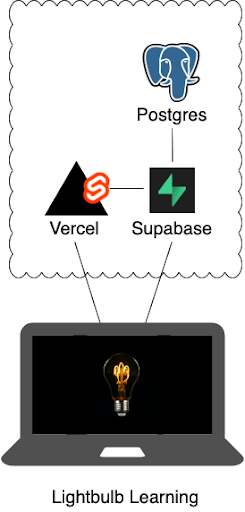
\includegraphics[width = .3\textwidth]{images/arch.png}
    \caption{High-level Architekturübersicht Lightbulb Learning}
    \label{fig:arch}
\end{figure}

In Abbildung \ref{fig:arch} werden die grundlegend verwendeten Technologien dargestellt. Die Endnutzer greifen mittels eines Browsers auf die Server von Vercel zu, welche das Frontend ausliefern und anhand von SSR einen Teil der Anfragen direkt im Server durchführen. Dazu gehören auch Zugriffe auf die Datenbank, welche als PostgREST API\footnote{\url{https://postgrest.org/en/stable/}} von Supabase bereitgestellt wird. Supabase betreibt und verwaltet für die Datenhaltung eine Instanz einer PostgreSQL-Datenbank\footnote{\url{https://www.postgresql.org/}}. Die folgenden Abschnitte gehen im Detail auf die Schnittstellen und Verantwortungsbereiche dieser Technologien ein.

\section{Supabase}
Supabase spielt in der Entwicklung von Lightbulb Learning eine zentrale Rolle, kann sogar als Schlüsseltechnologie bezeichnet werden. Eine Beschreibung der Aufgaben, die Supabase direkt und durch die Bereitstellung einer PostgreSQL Datenbank übernimmt, wird in den folgenden Abschnitten beschrieben.

\subsection{Vergleich: Supabase und Firebase}
Supabase beschreibt sich selbst als Open-Source Alternative zu Firebase\footnote{\url{https://firebase.google.com/}}, welche „die Features von Firebase mithilfe von Enterprise-tauglichen Open-Source Tools”\cite{supabase} nachbaut. Diese Funktionalitäten sind, neben einem zugänglichen Dashboard, im Wesentlichen die Bereitstellung einer Datenbank hinter einer im Internet verfügbaren Schnittstelle (bei Bedarf mit Echtzeit Subscriptions). Zusätzlich wird die Verwaltung der Authentifizierung und Autorisierung für die Zugriffe auf diese API und auf die dahinterliegenden Daten abgebildet. Auch die Möglichkeit, Dateien in einem Bucket abzulegen und Funktionen, welche auf dem Datenbankserver ausgeführt werden, wird zur Verfügung gestellt.. Dabei geht Supabase einige Aspekte auch anders als die eigens genannte Inspirationsquelle Firebase an, um weitere Mehrwerte neben dem Open-Source Gedanken anbieten zu können. Anstelle der dokumentenorientierten Datenstruktur in Firebase wählt Supabase ein relationales Datenmodell. Ein weiterer großer Unterschied ist die Art und Weise, wie auf die Daten zugegriffen wird. In Firebase gibt es dazu eine Frontend-Bibliothek, welche diese Aufgabe übernimmt, dabei allerdings sowohl intransparenter als auch weniger flexibel als der Client in Supabase ist. Während die Frontend-Bibliothek von Supabase im Wesentlichen lediglich eine JavaScript-Repräsentation der Abfragesprache übernimmt und diese den entsprechenden REST Aufrufe zuweist, ist bei Firebase Firestore der präferierte Weg vom Browser zur Datenbank immer den offiziellen Client zu verwenden. Dieser Client behält sich vor, die Datenstruktur sowie auch die Schnittstelle in Richtung der Datenhaltung zu verändern, so dass hier keine eigene Implementation für diese Aufgabe begünstigt wird. Die bestehende Implementierung ist dabei gleichzeitig nicht für den Einsatz auf der Serverseite ausgelegt, so dass die Entwicklung einer Applikation mit Server-Side Rendering deutlich erschwert wird. Für die Entwicklung nativer Applikationen werden entsprechend Bibliotheken bereitgestellt, um auch dies zu ermöglichen. Aufgrund dieser inhaltlichen Unterschiede zeigt sich, dass Supabase nicht nur eine Firebase Alternative ist, sondern lediglich ein Teil der gleichartigen Probleme adressiert. Gleichzeitig ist die Parallele zwischen den beiden Technologien aus der Perspektive des Marketings für Supabase ein sehr guter Ansatz, um Entwicklern und potentiellen Kunden, denen Firebase häufig schon ein Begriff ist, sehr schnell zu vermitteln, welches Problem Supabase löst.
\subsection{Relationale Datenbanken}
Welche Eigenschaften eine relationale Datenbank für den Anwendungsfall einer Applikation mit strukturierten Daten nützlich macht, soll in diesem Abschnitt diskutiert werden. Grundsätzlich ist die Idee einer relationalen Datenstruktur die Verbindung von Zeilen unterschiedlicher Tabellen anhand von Schlüsseln, welche eindeutige Zuweisungen ermöglichen. Dadurch kann eine Abfragesprache genutzt werden, welche die Zusammenhänge zwischen mehreren Tabellen beachtet oder diese zur Abfragezeit nach Bedarf miteinander kombiniert. Die relationale Datenbank garantiert dabei die Eigenschaften der Atomarität, Konsistenz, Isolation und Dauerhaftigkeit von Änderungen, dies wird üblicherweise mit dem Akronym ACID abgekürzt. Atomarität bedeutet, dass eine Transaktion stets entweder komplett durchgeführt wird, oder, im Falle des Scheiterns einer Transaktion, der ursprüngliche Zustand vollständig wiederhergestellt wird. Die Aufrechterhaltung der Konsistenz bedeutet, dass die Relationen zwischen den einzelnen Tabellen zu jedem Zeitpunkt entsprechend der formulierten Regeln (und somit intakt) gehalten wird. Die Isolation ist auf der zeitlichen Achse zu betrachten: Ist eine Transaktion noch nicht beendet, so können die Änderungen, die innerhalb dieser Transaktion stattfinden, nicht von einer parallel stattfindenden Transaktion gelesen werden. Die Änderungen sind somit so lange voneinander isoliert, bis eine Transaktion erfolgreich abgeschlossen wurde. Die Dauerhaftigkeit von Daten beschreibt, dass die Daten einer erfolgreichen Transaktion auf einer Festplatte persistiert werden. Wird das System beispielsweise von der Stromversorgung getrennt und zu einem späteren Zeitpunkt wieder angeschlossen, so sind die vorher gespeicherten Daten immer noch verfügbar.
\subsection{PostgreSQL (alias Postgres)}
Supabase betreibt eine PostgreSQL bzw. Postgres Datenbank (beide Bezeichnungen werden austauschbar verwendet \cite{PagePostgres}). PostgreSQL ist eine etablierte relationale Datenbank, welche seit dem ersten öffentlichen Release 1996 aktiv von der Open Source Community weiterentwickelt wird. Der Fokus dabei liegt auf der Zuverlässigkeit, Datenintegrität, Erweiterbarkeit, Performanz und Skalierbarkeit \cite[vgl.][]{PostgresAbout}. Gleichzeitig verfügt PostgreSQL über eine Vielzahl an Features\footnote{\url{https://www.postgresql.org/about/featurematrix/}}, von denen einige im Kontext der Serverless-Anwendungsentwicklung sich als besonders nützlich erweisen. Dazu zählen insbesondere die PostgreSQL Row-Level-Security Regeln (RLS) und die PostgreSQL Functions, welche in den folgenden Abschnitten erläutert werden.
\subsection{Row-Level-Security}
Die Row-Level-Security Funktionalität von PostgreSQL\footnote{\url{https://www.postgresql.org/docs/current/sql-createpolicy.html}} kann für die Definition von Zugriffsregeln auf die Daten genutzt werden. In Abbildung \ref{fig:rls} ist ein Beispiel aus Lightbulb Learning für den lesenden Zugriff auf die Tabelle course\_user. Die Definition der Regel ist seinerseits eine SQL-Abfrage, welche einen Wahrheitswert, welcher über die Blockierung der weiteren Durchführung entscheidet, zurückgibt.
\begin{figure}[H]
    \centering
    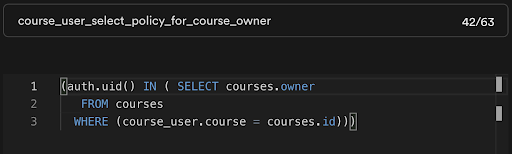
\includegraphics[width = .8\textwidth]{images/prls.png}
    \caption{Row-Level-Security-Regel Beispiel für Kurs-Besitzer}
    \label{fig:rls}
\end{figure}
\noindent In diesem Beispiel ist das SQL Statement wahr, falls der anfragende User als Besitzer des Kurses gelistet ist. Für die Teilnehmer des Kurses ist eine weitere Regel hinterlegt, da sich die Anfragen inhaltlich unterscheiden. Die Verwendung von Row-Level-Security Regeln erweist sich als gangbare Alternative zur Entwicklung eines eigenen Backends zur Verwaltung der Zugriffsrechte auf Zeilenebene der Datenbank, da diese Komplexität eingespart werden kann, gleichzeitig aber die Feinheit der Granularität der Zugriffsregeln beliebig gesteigert werden kann. Für noch komplexere Regeln oder die Wiederverwendung von Strukturen können auch PostgreSQL Functions genutzt werden. Diese werden im Folgenden Abschnitt erläutert.
\subsection{PostgreSQL Functions}
\label{sub:sqlfunc}
Das Feature von PostgreSQL Functions\footnote{\url{https://www.postgresql.org/docs/current/sql-createfunction.htm}} bietet die Möglichkeit, serverseitigen Code auszuführen, ohne dabei die Laufzeitumgebung oder andere zusätzliche infrastrukturelle Aspekte neben der Datenbank selbst verwalten zu müssen. Da der Code direkt auf der Datenbank ausgeführt wird, können die definierten Rollen (im Sinne der Autorisierung) verwendet werden, um sicherheitsrelevante Abfragen zu machen. Dies ist beispielsweise dann von Belang, wenn private Token verwendet werden, welche nicht an den Client ausgeliefert werden dürfen. Ein zweiter Anwendungsfall ist die Wiederverwendung von Logik in unterschiedlichen Kontexten, etwa bei der Definition von Row-Level-Security Regeln. Ein weiterer Anwendungsfall ist die die Einbeziehung von äußeren Faktoren in eben solche Regeln, welche nicht in Form von einer SQL Abfrage abbilden lassen. Ein Beispiel für diesen Fall findet sich in der folgenden Abbildung \ref{fig:func}.
\begin{figure}[H]
    \centering
    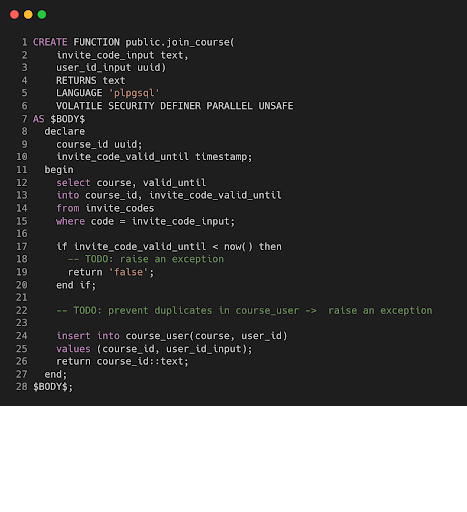
\includegraphics[width = .8\textwidth]{images/pfun.png}
    \caption{Die join\_course Funktion}
    \label{fig:func}
\end{figure}
\noindent Zuerst fällt die etwas umständliche und unflexible Definition der Funktion auf, welche der verwendeten Sprache PL/pgSQL geschuldet ist. Dies steht für Procedural Language/Postgres Structured Query Language und erweitert SQL um unter anderem um Variablen, Bedingungen und Schleifen in Form einer prozeduralen Sprache\footnote{\url{https://www.postgresql.org/docs/current/plpgsql-structure.html}}, welche bereits 1998 erschienen ist. Für einfachere Fälle ist es auch möglich, PostgreSQL Functions in SQL zu schreiben, falls diese Spracherweiterungen nicht benötigt werden. Im Beispiel wird in den Zeilen 1-6 der Kopf der Funktion selbst definiert. Dazu gehören der Name, die Eingabeparameter, die verwendete Sprache und der Rückgabewert. Die Zeilen 8-10 definieren die verwendeten Variablen, welche im eigentlichen Rumpf der Funktion, also in den Zeilen 12-26, verwendet werden dürfen. Hier wird zu einem bestimmten Einladungscode der Ablaufzeitpunkt mit dem aktuellen Zeitpunkt verglichen. Ist der Einladungscode noch nicht abgelaufen, so wird der Nutzer dem entsprechenden Kurs hinzugefügt und der Primärschlüssel des Kurses zurückgegeben. Da dieses Beispiel sowohl die Möglichkeiten dieser prozeduralen Spracherweiterung, als auch die damit einhergehenden Schwierigkeiten besonders plakativ darstellt, wird im Kapitel \ref{chap:eval} dazu detaillierter Stellung bezogen. Auch wenn Seiteneffekte in Form von Zustandsänderungen der Datenbanktabellen ein natürlicher Effekt von PostgreSQL Functions sind, so kann doch durch die Anwendung von Transaktionalität auf SQL-Ebene der Umgang mit Fehlern eindeutig geregelt werden, beispielsweise durch die Durchführung eines Rollbacks in diesem Fall. Nachdem eine Funktion definiert ist, wird sie von Supabase in der API zur Verfügung gestellt \cite[vgl.][]{SupabaseFunctions}, und kann vom Client aus direkt aufgerufen werden.
\subsection{PostgREST}
PostgREST ist eine Serveranwendung, welche eine generische Zuordnung zwischen den relationalen Datenstrukturen und -operationen der PostgreSQL-Datenbank und dem  \cite[Kapitel 5]{fielding00} vornimmt. So kann beispielsweise für das Löschen einer Zeile in der Datenbank ein REST DELETE genutzt werden. Dabei wird eine Referenz auf eine Ressource (aus REST Sicht), welche dem Primärschlüssel der Zeile in der PostgreSQL Datenbank entspricht, zur Identifikation des zu löschenden Elements angegeben. In Abbildung \ref{fig:delete} wird beispielsweise das Löschen eines Kurses durch einen HTTP Aufruf dargestellt. Die Anfragemethode ist in diesem Beispiel DELETE, während die Id, also der Primärschlüssel des Kurses, als Anfrageparameter übergeben wird.
\begin{figure}[H]
    \centering
    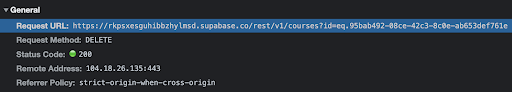
\includegraphics[width = .9\textwidth]{images/rest.png}
    \caption{Screenshot der Netzwerküberwachung in Chrome beim Löschen eines Kurses}
    \label{fig:delete}
\end{figure}
\noindent PostgREST identifiziert diesen API-Aufruf als Löschanfrage, übersetzt es in die entsprechende SQL Anfrage und führt diese auf der PostgreSQL-Datenbank aus. Ist die SQL Anfrage erfolgreich, so wird wiederum der entsprechende Status Code 200 zurückgegeben. Das gleiche Muster funktioniert ebenfalls für das Anlegen, Auslesen und Verändern von Elementen mit den jeweiligen REST und SQL Äquivalenten. PostgREST ermöglicht mittels der Definition von Konfliktlösungs- und Verschmelzungsstrategien sowie der Kombination von Anfrageparametern die Möglichkeit, auch komplexere Anfragen durchzuführen, ohne dafür eine serverseitige Applikation schreiben, testen, betreiben und skalieren zu müssen. Damit fügt sich die Kombination aus PostgREST und PostgreSQL mit seinen Funktionen wie Row-Level-Security und Functions, als gehostete Dienstleistung von Supabase, in den Komplex einer Serverless-Anwendung ein.
\section{Web Applikation mit SvelteKit}
Entsprechend der Anforderung der hohen Entwicklungsgeschwindigkeit und größtmöglichen Flexibilität fiel die Entscheidung zwischen den zur Verfügung stehenden Frontend-Frameworks wie beispielsweise VueJS\footnote{\url{https://vuejs.org/}}, Angular\footnote{\url{https://angular.io/}} und React\footnote{\url{https://reactjs.org/}} auf ein sehr modernes Framework namens SvelteKit\footnote{\url{https://kit.svelte.dev/}}.
\subsection{SvelteKit und Svelte}
SvelteKit wird auf der eigenen Homepage als Framework für Webapplikationen jeder Größe, mit einem flexiblen Dateisystem-basierten Routing beschrieben. Es funktioniert so, dass man, ähnlich wie bei den übrigen verbreiteten Frameworks auch, Komponenten als Dateien in einem eigenen Format beschreibt. Streng genommen muss man dabei zwischen SvelteKit und Svelte\footnote{\url{https://svelte.dev/}} unterscheiden. Svelte ist das von SvelteKit genutzte Komponenten-Framework, dessen Aufgabe es ist, aus Interaktivität, Struktur und Styling bestehende Komponenten zur Kompilierungszeit in hoch optimiertes JavaScript mit HTML und CSS zu kompilieren. Dies gelingt über die Ausnutzung der labelled Syntax in der Sprachdefinition von JavaScript, durch welche dynamische Abhängigkeiten zwischen Variablen ausgedrückt werden können \cite[vgl.][]{svelteReactive}, was wiederum den Verzicht auf das Virtual DOM ermöglicht \cite[vgl.][]{Harris2018}. Neben der Nutzung optimierter Svelte-Komponenten folgt SvelteKit einem weiteren, sehr mächtigem Prinzip, nämlich dem der Transitional Apps. Um dieses zu erklären, ist es wichtig, sich die deutlich verbreiteteren Begriffe der Multi-Page Application (MPA) und der Single-Page Application (SPA) vor Augen zu führen.
\subsection{Multi-Page Apps (MPAs)}
Multi-Page Applications sind der traditionelle Weg der Auslieferung von Web-Applikationen. Dabei werden Routen auf Ressourcen gemappt, welche mit voneinander separaten Aufrufen vom Browser aus abgefragt und dargestellt werden. Dieser Vorgang kann auch durch Server-Side Rendering (SSR) unterstützt werden, welches die ausgelieferte HTML-Datei anhand von Anwendungslogik auf dem Server zusammensetzt. Dieses Vorgehen hat einige Vorteile. Wird eine Ressource aufgerufen, so kann diese ohne weitere Zwischenschritte direkt und schnell, optional sogar ohne JavaScript-Anteile, ausgeliefert werden. Die Anwendungslogik kann im Server abgebildet werden, so dass Entwickler eine größere Auswahl an Technologien zur Verfügung haben. Des Weiteren können die Features des Browsers, wie beispielsweise die Navigationselemente, so genutzt werden, wie sie ursprünglich gedacht waren: Zum Navigieren zwischen den Seiten. Es bestehen allerdings auch einige Nachteile: Zwischen den einzelnen Aufrufen kann kein Zustand geteilt werden, was bedeutet, dass beispielsweise bei der Verwendung von JavaScript-Bibliotheken sämtlicher Code neu geladen und evaluiert werden muss. Dies verlangsamt die Navigation innerhalb einer Web-Applikationen spürbar, auch deshalb, weil jede neue Seite einzeln über das Netzwerk übertragen werden muss. Auch für Designprinzipien wie das der Objektpermanenz sind Multi-Page Apps schlichtweg nicht ausgelegt, so dass visuelle Transitionen zwischen zwei unterschiedlichen Seiten unmöglich werden.
\subsection{Single-Page Apps (SPAs)}
Der modernere Ansatz der Single-page Applikationen löst einige dieser Probleme, erzeugt dabei aber zugleich einige neue Nachteile. Die Grundidee von SPAs ist, dass sämtliche für die Darstellung der Applikation notwendigen Aspekte beim initialen Laden der Webseite heruntergeladen und gecached werden. Durch die Benutzer-Interaktion wird das DOM direkt im Browser manipuliert, ohne dabei eine weitere Seite mit den üblichen Browser-Mechanismen zu laden. Dadurch wirken SPAs, nach einer etwas verlängerten initialen Ladezeit, sehr schnell und weisen daher beispielsweise bei der Web-Applikation internen Navigation Ähnlichkeiten mit lokal installierten Applikationen auf. Allerdings stößt man durch die Anwendung dieses Prinzips auch sowohl auf Grenzen, etwa beim Laden dynamischer Inhalte welche unmittelbar mit Eingaben des Nutzers zusammenhängen, als auch auf konkrete Nachteile, wie die erhöhte initiale Ladezeit beim Aufruf einer Webseite. Zusätzlich wird das Routing in einer SPA virtualisiert, womit eine gewisse Fehleranfälligkeit einhergeht. Außerdem bedeutet es, dass das Öffnen einen Deeplinks dazu führt, dass die gesamte Applikation anstelle der eigentlich angefragten Ressource geladen werden muss. Innerhalb dieser Applikation muss dann die ursprünglich angefragte URL als Eingabeparameter gedeutet werden, und die entsprechenden Inhalte müssen dargestellt werden. Dadurch wird die Umsetzung von Deeplinks nicht nur deutliche verlangsamt, sondern auch zu einem expliziten, optionalen und fehleranfälligem Feature einer SPA, es ist entsprechend also denkbar, dass eine Web-Applikation Deeplinks überhaupt nicht unterstützt.
\subsection{Transitional Apps}
SvelteKit befolgt das Prinzip der Transitional Apps \cite[vgl.][]{Harris2021}. Dieser Begriff ist noch sehr jung und wenig in den einschlägigen Referenzen verankert, beschreibt aber treffend den Umgang mit den Abwägungen, die zwischen MPAs und SPAs gemacht werden müssen. Es soll widergespiegelt werden, dass die Vorteile beider Prinzipien, sowohl der traditionellen, als auch der modernen, kombiniert werden. Ursprünglich stammt der Begriff aus dem Interior Design und wird als „blend of traditional styles with the contemporary styles of the day” \cite{Wearstler2022}, also einer Kombination aus traditionellem und zeitgenössischem Stil beschrieben. Die Übertragung dieser Begrifflichkeit und dem dahinter liegenden Prinzip bedeutet: Eine transitionale App ist einerseits vorwärtsgewandt und hat einen Blick auf die Vorteile der Lösungen, die eine SPA anbieten, respektiert aber gleichzeitig die Vorteile der traditionellen MPAs, und versucht insgesamt, die Vorteile beider Prinzipien miteinander zu kombinieren \cite[vgl.][]{Harris2021}. 
\subsection{Adapter, Server-Side Rendering und Hydration}
SvelteKit erreicht dieses Ziel unter anderem durch sogenannte Adapter\footnote{\url{https://kit.svelte.dev/docs/adapters}}, welche für SvelteKit Projekte konfigurierbar sind. Die Aufgabe eines Adapters ist die Umwandlung einer kompilierten SvelteKit-Applikation in ein Deployment-Paket, welches für eine bestimmte Deployment-Umgebung ausgelegt ist. Dadurch kann der Einsatz von Server-Side Rendering lose von unterschiedlichen Deployment-Providern und den jeweils verwendeten Laufzeitumgebungen gewährleistet werden. Beispiele für Deployment-Provider, für welche solche Adapter bereits existieren, sind Vercel\footnote{\url{https://vercel.com/}}, Netlify\footnote{\url{https://www.netlify.com/}} und Cloudflare\footnote{\url{https://www.cloudflare.com/}}. Durch das Server-Side Rendering können Komponenten, welche nur aus statischen Anteilen bestehen, vorgerendert und dadurch ohne weitere Zwischenschritte direkt ausgeliefert werden können. Komponenten mit dynamischen Aspekten werden zur initialen Anfragezeit vorerst als statisches HTML-Dokument ohne Interaktivität provisioniert. Gleich im Anschluss daren werden benötigte dynamische Anteile nachgeladen, so dass die Seite nicht nur dargestellt, sondern auch damit interagiert werden kann. Dieser Prozess der Hydration\footnote{\url{https://kit.svelte.dev/docs/page-options\#hydrate}} ist für den Nutzer nicht sichtbar, führt aber in seiner Wahrnehmung zu sehr kurzen initialen Ladezeiten. Im Anschluss lädt SvelteKit die Seiten vor, welche von der aktuellen Seite aus direkt erreicht werden können. Dies führt dazu, dass bei der Navigation zu anderen Seiten innerhalb der Transitional App der interne Router von SvelteKit die Steuerung der Browser-Navigation übernehmen kann. Dadurch kann auf die zusätzliche Fehleranfälligkeit, welche durch die Umsetzung dieser Funktionalität durch den App-Entwickler selbst entstehen würde, verzichtet werden. In diesem Kontext werden Frameworks, welche diese Aufgaben übernehmen, werden auch Meta-Frameworks genannt. Alternativen wären beispielsweise Nuxt\footnote{\url{https://nuxtjs.org/}} für Vue und NextJS\footnote{\url{https://nextjs.org/}} für React.
\section{TypeScript}
Für die Entwicklung der Applikation wurde insbesondere TypeScript\footnote{\url{https://www.typescriptlang.org/}} verwendet. TypeScript ist eine Erweiterung von JavaScript, welche von Microsoft weiterentwickelt und als JavaScript mit der Syntax für Typen beworben wird. Die stark typisierte Sprache bietet einen umfassenden Satz an Werkzeugen für die Entwicklungsumgebung, welche die Entwicklung beschleunigen und die Fehlerwahrscheinlichkeit zur Laufzeit verringern, indem es Typen eindeutig macht und Fehler bereits zur Kompilierzeit aufdeckt. Dadurch erhöht sich auch die Testbarkeit der Applikation, da durch die Typisierung nach der Kompilierung mehr über die Objekte bekannt ist, und somit die Anzahl der möglichen Fälle bekannt. Da Browser lediglich JavaScript Code ausführen können, wird der TypeScript Code zu optimiertem JavaScript transpiliert. Da sowohl TypeScript, als auch die etablierte Entwicklungsumgebung Visual Studio Code als open source Projekte von Microsoft verwaltet werden, sind diese gut miteinander integriert.
\section{Skalierung der Datenbank}
Für die Analyse der Antwortbereitschaft von Lightbulb Learning ist die Datenbank als einzige zentrale Instanz als Flaschenhals für die Skalierung im Erfolgsfall zu sehen. Daher stellt sich die Frage, ob man eine PostgreSQL-Datenbank so skalieren kann, dass für alle Kunden eine positive Benutzererfahrung erhalten bleibt. Darauf hat die PostgreSQL-Datenbank und dessen Community einige Antworten, welche sowohl im Bereich der vertikalen, als auch in der horizontalen Skalierung liegen. Die vertikale Skalierung entspricht der Erhöhung der Ressourcen für eine einzelne Instanz. Für die Benutzung durch Supabase entspräche das dem Upgrade von der Free auf die Pro Version, wobei hier auch teilweise Elemente der horizontalen Skalierung enthalten sind). Als relevantere Frage ergibt sich somit: Was, wenn die horizontale Skalierfähigkeit von PostgreSQL durch Supabase limitiert wird? In dem Fall könnten die Daten mit einem einfachen Befehl aus Supabase extrahiert werden, und eine eigene Datenbank-Infrastruktur aufgebaut werden. In dieser könnten dann alle Konzepte der horizontalen Skalierung angewendet werden, welche auf der Ebene von PostgreSQL ermöglicht werden. Für Applikationen, welche überwiegend lesende Zugriffe auf die Datenbank machen, wie das bei Lightbulb Learning der Fall ist, wird empfohlen, weitere Replicas hinzuzufügen, auf welche die Lesezugriffe aufgeteilt werden können. Würde die Applikation mit der Menge an Schreibzugriffen an ein Limit stoßen, so kann die Datenbank auf mehrere Server partitioniert werden, indem entweder unterschiedliche Tabellen auf unterschiedlichen Datenbankservern gehalten werden, oder sogar eine einzige Tabelle auf mehrere Server mittels Sharding aufgeteilt wird. Dennoch gibt es auch hier eine Grenze, welche durch die Erhaltung der Konsistenz Garantie entsteht. Die Wahrscheinlichkeit des Eintretens dieser Bedarfe ist zwar sehr gering, aber dennoch ist es allgemein eine sinnvolle Absicherung, im Erfolgsfall einen Plan zu haben, die technische Infrastruktur mit sprunghafter Nachfrage skalieren zu können. Supabase in Kombination mit PostgreSQL ermöglichen die Umsetzung dieses möglichen Bedarfs.
\section{Testing mit Playwright}
Für das Testen von Lightbulb Learning wird Playwright\footnote{\url{https://playwright.dev/}} verwendet, einem von Microsoft betreuten open source Werkzeug zur Testautomatisierung, welches bei der Initialisierung von SvelteKit Projekten mit dem CLI Tool als Standard Testing-Framework vorgeschlagen wird. Mit Playwright lassen sich Anwendungsfälle durch die direkte Interaktion mit dem Browser testen und debuggen, die Tests entsprechen also echten Ende-zu-Ende Tests. Dadurch können die Tests gegen eine Produktivumgebung ausgeführt werden. Die Möglichkeit, die Tests mit unterschiedlichen Browsern auszuführen, so dass auch hier Bugs aus Nutzersicht früh entdeckt und gelöst werden können, erhöht verringert zusätzlich die Wahrscheinlichkeit für blinde Flecken. Im Gegensatz zu Cypress\footnote{\url{https://www.cypress.io/}}, einem konkurrierenden und zu Beginn des Projekts verwendeten Testframework, können durch die Verwendung der modernen async/await Strukturen und automatischen Retries resiliente und aussagekräftige Tests geschrieben werden, die sich auf unterschiedlich schnellen Umgebungen gleich Resultate liefern. Das Besondere an diesen Tests ist aber, dass sie die Funktionen des Systems aus Nutzersicht beschreiben, und als lebende Dokumentation dessen betrachtet werden, was das System zum Zeitpunkt des Ausführung wirklich zu tun vermag. Ist ein bestimmter Test erfolgreich, so ist damit unter Voraussetzung korrekter Implementierung des Tests validiert, dass das System eine gewünschte Eigenschaft erfüllt. Schlagen Tests fehl, so ist das Gegenteil der Fall, und es muss etwas dafür getan werden, dass die gewünschten Eigenschaften wieder erfüllt werden. Dieses Prinzip wurde bereits 2006 im Artikel über Behavior-Driven Development \cite[vgl.][]{North2006} (BDD) von Dan North erläutert.
\section{Continuous Deployment Pipeline mit GitHub Actions}
Für die Kompilierung, automatische Testausführung und automatische Deployments wurde eine Continuous Deployment Pipeline mit GitHub Actions\footnote{\url{https://github.com/features/actions}} aufgebaut, welche durch Interaktion mit der Versionsverwaltung ausgelöst wird. Jeder Commit führt zur automatischen Durchführung aller Tests (unabhängig vom Branch), dafür wird auf dem GitHub Actions Server eine lokale Datenbank gestartet und mit Testdaten initialisiert, der Entwicklungsserver gestartet, der das Frontend ausliefert und im headless Modus die definierten Anwendungsfälle getestet. Bei GitHub Actions handelt es sich ebensfalls um eine Serverless-Technologie. Schlägt mindestens ein Test fehl, wird eine Mail mit einem Fehlerprotokoll versendet. Unabhängig vom Testergebnis wird daraufhin ein Preview-Deployment auf Vercel durchgeführt, so dass jede Version der Applikation bei Bedarf unter realistischen Bedingungen manuell getestet werden kann. Die einzige Ausnahme dafür sind Commits, welche auf den main branch gepusht werden: Diese werden automatisiert auf die Produktivumgebung deployed.